\subsection{Initial Graphics Exchange Specification (IGES) file}
\paragraph{}
In the proposed approach, the geometry will be imported from the IGES file.
IGES file can be easily exported from almost all popular CAD softwares such as AutoCAD.
In this section, we give a brief overview of IGES file format.
For more detailed description and implementation aspects, interested readers can refer to \cite{uspro2006}.

\subsubsection{General data form}
\paragraph{}
A typical IGES file will be divided into 5 sections: start section, global section, directory entry section, parameter data section and terminate section as shown in Fig.~\ref{lr_fig:iges_data_form}

\paragraph{Start section}
The start section provides a human-readable description about the file.
This section will always have the letter `S' in 73rd column.
Data filed of the start section will starts at column 1 and ends at column 72.
The filed can contain any text message expect ASCII control characters.
Start section must appear in the file.
The text can be empty but the sequence filed shall not left empty.

\paragraph{Global section}
The global section describe the preprocessor and information that are necessary to handle the file by post-processors.
Similar to start section, global section will always have the letter `G' in 73rd column.
Parameters for the global section will be discussed later.

\begin{figure}[!ht]
    \centering
    \scalebox{0.4}{
        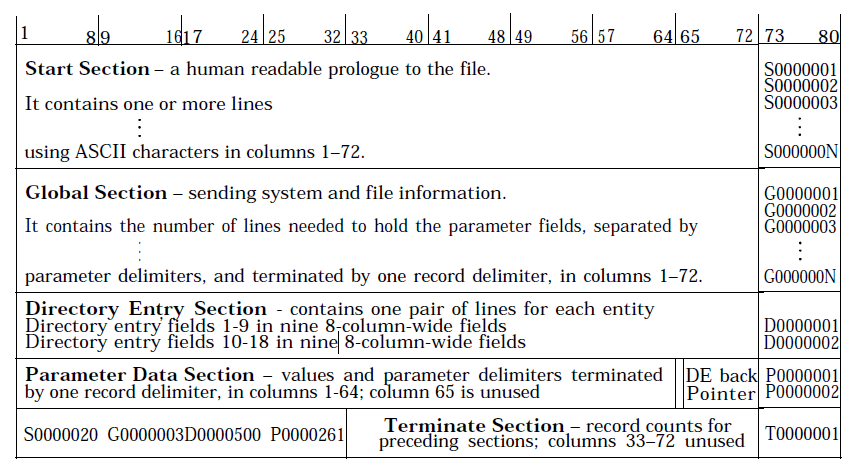
\includegraphics{literature/images/lr_iges_data_form.png}
    }
    \caption{File structure of an IGES file}
    \label{lr_fig:iges_data_form}
\end{figure}